\chapter{Design del Protocollo}
\label{chap:design_protocollo}
\section{Architettura generale del sistema}
\begin{figure}[H]
    \centering
    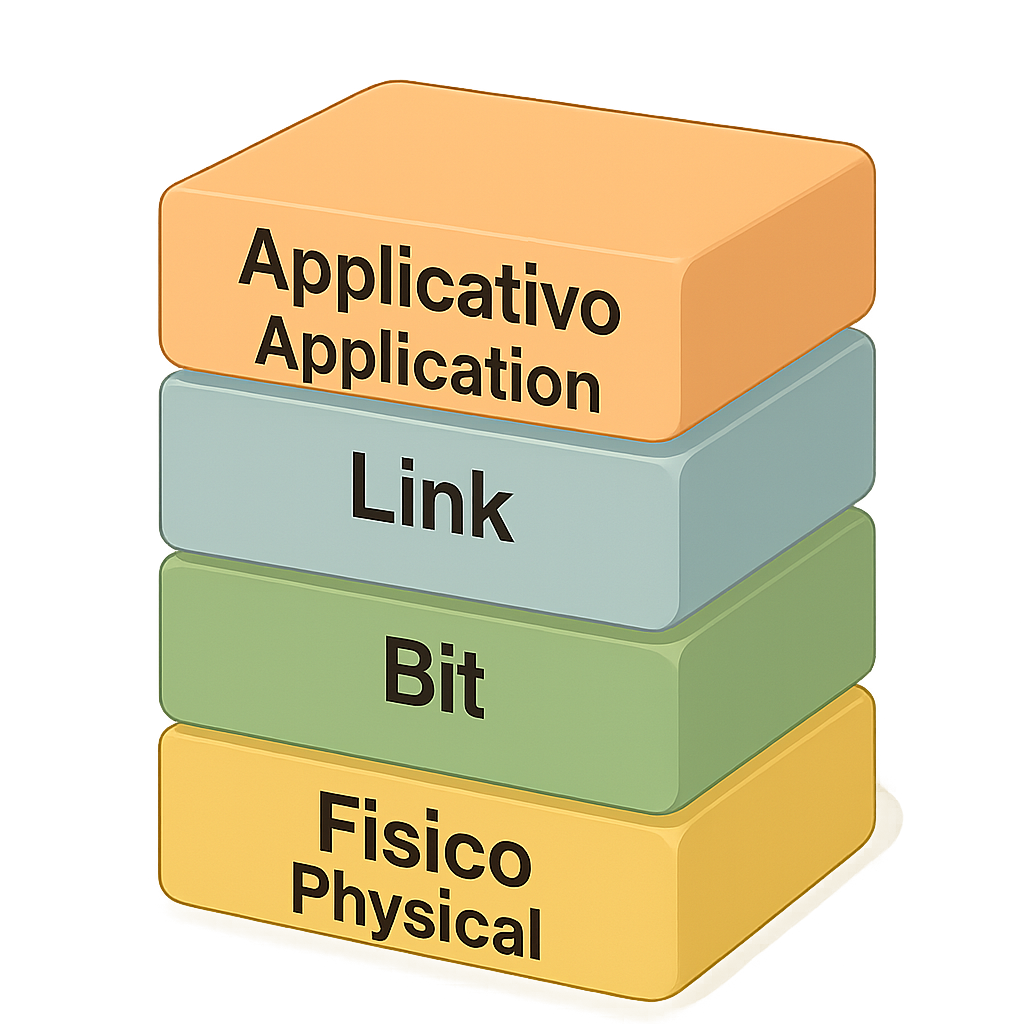
\includegraphics[width=0.35\textwidth]{immagini/layers.png}
    \caption{Livelli del Protocollo}
    \label{fig:esempio}
\end{figure}
Il protocollo è strutturaro in quattro livelli principali, ognuno con una funzione specifica.
\section{Livello Fisico}
Il livello fisico è responsabile della tramissione dei bit precedentemente composti dal livello Bit.
Questo sfrutta uno speaker per la trasmissione e un microfono per la ricezione dei bit che vengono trasmessi mediante coppie superimposte di frequenze.
\subsection{Ingresso}
Il microfono I2S è collegato al microcontrollore ESP32 tramite il bus I2S, sfruttando uno dei due canali disponibili.  
Il segnale audio viene campionato a $48\,\text{kHz}$ con una risoluzione di 16 bit, per poi essere gestito mediante due array in swapping, concetto che verrà approfondito successivamente. \\

\noindent
La scelta della frequenza di campionamento deriva dal \textbf{teorema di Nyquist-Shannon} \cite{shannon1949}, secondo il quale un segnale può essere ricostruito senza ambiguità se la frequenza di campionamento $f_s$ è almeno doppia rispetto alla massima frequenza del segnale $f_{\max}$:
\[
f_s \geq 2 f_{\max}.
\]
Ne consegue che la massima frequenza rappresentabile è
\[
f_{\text{Nyquist}} = \frac{f_s}{2}.
\]

Nel nostro caso:
\[
f_s = 48\,\text{kHz} \quad \Rightarrow \quad f_{\text{Nyquist}} = 24\,\text{kHz}.
\]

Poiché l’orecchio umano percepisce frequenze fino a circa $20\,\text{kHz}$ \cite{zwicker1999psychoacoustics}, la scelta di $48\,\text{kHz}$ garantisce la copertura dell’intero spettro udibile, con un margine di sicurezza di $4\,\text{kHz}$. Frequenze prossime al limite teorico di Nyquist risulterebbero invece difficili da catturare senza aliasing, a causa dei limiti pratici dei filtri anti-alias. \\

\noindent
Per l’elaborazione, i campioni vengono raccolti in blocchi di lunghezza $N = 512$. Con la frequenza di campionamento fissata:
\[
T_{\text{blocco}} = \frac{N}{f_s} = \frac{512}{48 \cdot 10^3} \approx 0.01066\,\text{s}.
\]
Ogni blocco di dati rappresenta quindi un intervallo di circa $10.7\,\text{ms}$ di segnale audio.  

\noindent
Una volta acquisito il blocco, viene calcolata la \textbf{trasformata veloce di Fourier (FFT)} \cite{cooley1965fft} per analizzare lo spettro in frequenza. La complessità della FFT cresce come $N \log_2 N$, e per $N=512$ si hanno circa:
\[
512 \cdot \log_2(512) = 512 \cdot 9 = 4608
\]
operazioni complesse.  

Sul microcontrollore ESP32 \cite{esp32techref}, operante a $120\,\text{MHz}$, questo si traduce in un tempo di elaborazione di circa $0.42\,\text{ms}$ per blocco, ovvero $\sim 0.83\,\mu\text{s}$ per campione. In termini di carico computazionale: $\sim 20$ moltiplicazioni, $\sim 29$ addizioni/sottrazioni e un’operazione di radice quadrata per campione, pari a $\sim 99$ cicli di clock.  

\noindent
Questo significa che, a fronte di una finestra temporale di $10.7\,\text{ms}$, l’FFT viene calcolata in meno del $5\%$ del tempo disponibile, consentendo un’elaborazione in tempo reale anche senza multi-threading.

\begin{figure}[H]
    \centering
    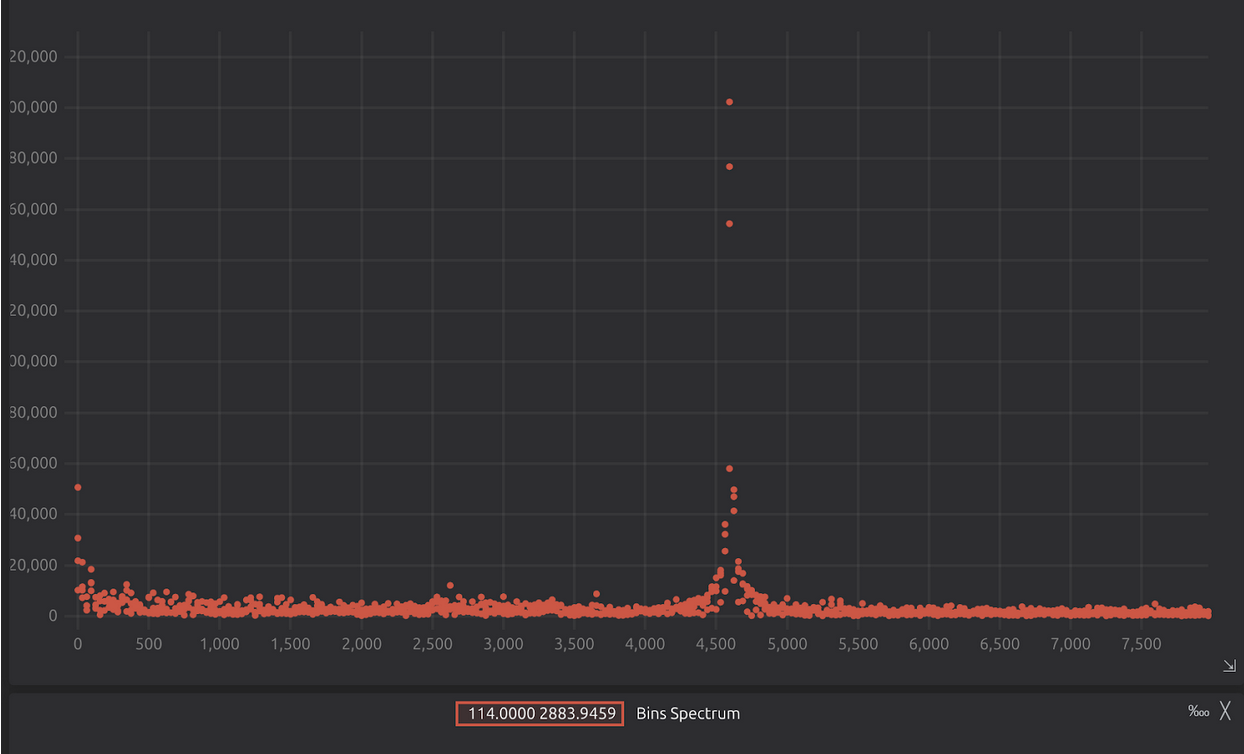
\includegraphics[width=0.9\textwidth]{immagini/fft_spectrum.png}
    \caption{Diagramma contentente lo spettro di frequenza calcolato tramite FFT} su un blocco di $512$ campioni acquisiti a $48\,\text{kHz}$.
    \label{fig:spettro}
\end{figure}

Come da Fig.~\ref{fig:spettro}, si può osservare che lo spettro di frequenza ottenuto dalla FFT mostra picchi alle frequenze di interesse, ma mostra anche un rumore di fondo.
Durante la creazione di questo protocollo sono emerse diverse difficoltà legate alla presenza di rumore ambientale,
questa condizione ha reso necessario l'uso di tecniche di filtraggio.
\subsection{Filtraggio}
L'idea iniziale, quando il protocollo era ancora nelle prime fasi di vita, era quella di utilizzare una semplice soglia fissa (filtro passa-basso) per discriminare i picchi dal rumore.
Tuttavia, questa soluzione si è rivelata inefficace, in quanto i microfoni presentano una risposta in frequenza che cala sulle alte, quindi i livelli in dB delle frequenze alte risultavano attenuati, non facendogli superare la soglia passa basso.
Inoltre, il rumore ambientale non è costante, ma varia nel tempo e nello spettro, rendendo difficile stabilire una soglia fissa che funzioni in tutte le condizioni.\\ 
Successivamente si è pensato di utilizzare delle soglie fisse, che variassero per ogni frequenza, in modo da tenere conto della risposta in frequenza del microfono.
Al fine di calcolare queste soglie, è stato utilizzato un algoritmo di \textit{regressione lineare} per stimare la retta che meglio approssima l'andamento della soglia minima:
\[
y = \beta_{} + \beta_{}x + \varepsilon \rightarrow y = -301.751324 \times x + 48531.689491
\]
Dove x rappresenta il numero del Bin.
